\section{Performances et validation}

Les calculs effectués sur les particules nécessitent une validation, afin de s'assurer que le comportement obtenu est conforme à la réalité physique. Une fois cette validation effectuée, nous avons pu réaliser quelques tests de performances, notamment pour vérifier que nos optimisations étaient eeffectives.

\subsection{Validation}

La validation est ici purement visuelle. En effet compte-tenu du dt qui peut varier entre chaque itération, et du nombre d'itérations, il  serait très difficile de comparer les positions de tout un lot de particule après notre simulation avec des données précalculées.

Nous nous somme donc focalisés sur deux exemples visuels simples qui sont des cas classiques de phénomènes physiques. Ces deux exemples se vérifient aisément puisque les trajectoires des particules des deux exemples sont très simples : rectiligne ou elliptique.

Pour la trajectoire rectiligne il s'agit de deux particules de même masse et sans vitesse ni accélération initiale. Elles s'attirent alors et se rapprochent l'une de l'autre avec une vitesse croissante. En ce qui concerne la trajectoire elliptique, il s'agit d'une particule de très grande masse sans vitesse ni accélération initiale associée à une particule de masse très faible avec une légère vitesse initiale orthogonale à la droite qui passent par les deux particules. La petite particule (i.e. de masse faible) effectue alors une trajectoire elliptique dont l'un des foyers est le centre de la grande particule.

\subsection{Etude des performances}

Nous avons effectué quelques benchmarks afin de mettre en avant les caractéristiques de notre implémentation du simulateur. Nous avons mis en avant la complexité de l'algorithme, montré qu'il était fortement parallélisable, et enfin nous avons mis en avant l'impact du dt variable sur les performances.

\subsubsection{Complexité}

La figure \ref{fig:complexity} montre bien que chaque c\oe ur effectue $pn^2$ opérations, car pour des valeurs moyennes, la courbe de $n^2$ a la même pente que les courbes de $T/p$ en fonction de $n$: $T/p = n^2$. Pour des grandes valeurs, au dessus de 128, la courbe possède un pic que nous n'arrivons pas à expliquer, mais qui s'est produit au même moment sur toutes les exécutions, et qui n'est donc pas de cause aléatoire. Par la suite, la courbe semble prendre une pente mois importante. Peut être s'agit-il de l'effet d'une optimisation.

\begin{figure}
\centering
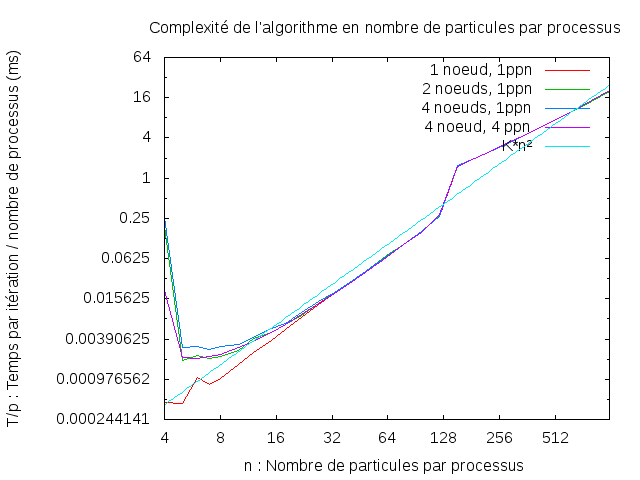
\includegraphics[scale=0.6]{complexity.png}
\caption{Complexité de la simulation}
\label{fig:complexity}
\end{figure}


\subsubsection{Parallélisation}

L'algorithme semble bien se comporter avec la parallélisation puisque les courbes de la figure \ref{fig:complexity} se confondent lorsque le nombre de particules est suffisant. En dessous de 16 particules par processus, la version la plus rapide est celle exécutée sur un seul processus, ensuite les courbes se confondent. Cela n'a rien d'étonnant puisque la taille des calculs croit de manière quadratique alors que celle des communications croit de manière linéaire et qu'en plus les communications sont recouvertes par le calcul.

On remarque aussi que pour n faible, la localité mémoire a son importance : la courbe violette a de meilleure performances bien qu'il y ait plus de processus car ces processus sont sur le même n\oe ud.


\subsection{\'Etude des performances de communications}

Pour vérifier que les calculs recouvrent bien les temps de communication, nous effectuons des calculs à charge égale (même nombre de processus, et de particules par processus) suivant plusieurs configurations possibles : 
\begin{itemize}
\item 1 n\oe ud utilisé avec 6 processus par n\oe ud (ppn) ;
\item 2 n\oe uds utilisés avec 3 ppn ;
\item 3 n\oe uds utilisés avec 2 ppn ;
\item 6 n\oe uds utilisés avec 1 ppn.
\end{itemize}

Si les calculs recouvrent les temps de communications, toutes les configurations devraient donc réaliser les calculs en un même temps, puisque ces configurations répartissent les calculs sur un nombre variable de n\oe uds donc nécessitant des temps de communications non négligeables. C'est ce que nous pouvons constater sur la figure \ref{img:nodes} où le temps de calcul en fonction du nombre de n\oe uds (mais avec un total de processus constant égal à 6) est une droite horizontale. Précisons que ces mesures ont été réalisées pour 10 particules, 10000 itérations et avec un dt automatique.

\begin{figure}
\centering
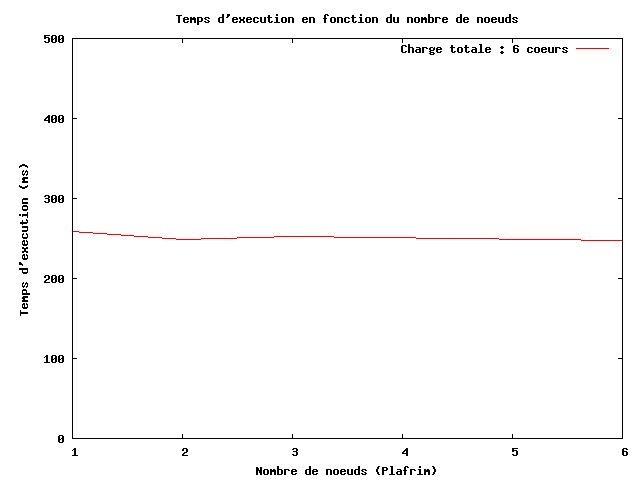
\includegraphics[scale=0.5]{img/graph_nodes.png}
\caption{Temps de calcul en fonction du nombre de n\oe uds impliqués.}
\label{img:nodes}
\end{figure}

\subsection{Comparaison avec un dt automatique}

L'introduction du dt automatique permet une plus grande précision dans les calculs mais nécessite une opération de calcul de racine d'un polynôme du second degré pour chaque particule. Il introduit donc nécessairement un léger surcoût, d'autant qu'il faut ensuite effectuer un \texttt{MPI\_ALLreduce} pour déterminer et communiquer le dt de la prochaine itération à tous les processus.

Cependant la complexité de ce calcul est ainsi linéaire en fonction du nombre de particules (avec toutefois un coefficient élevé), donc asymptotiquement il ne devrait pas induire une trop grande différence avec la version originale (avec un dt constant) puisque la complexité totale du problème est quadratique en le nombre de particules. La figure \ref{img:dt} semble pourant indiquer qu'au contraire l'écart de temps entre les deux versions se creuse, mais il faudrait effectuer ces mesures sur un plus grand nombre de particules pour en être certain.

\begin{figure}
\centering
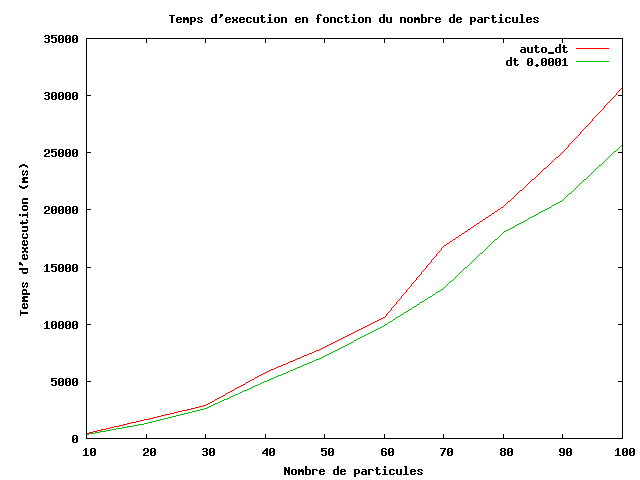
\includegraphics[scale=0.5]{img/graph_auto_dt.png}
\caption{Temps de calcul en fonction du nombre de particules.}
\label{img:dt}
\end{figure}

